\section{Architectuur}
\label{chapter:architecture}

\textit{
  In dit hoofdstuk wordt de vraag ``Uit welke componenten bestaat een Blockchain implementatie?'' behandeld. Het antwoord op deze vraag dient om een duidelijk beeld te scheppen welke componenten betrekking hebben op de onderdelen Distributed Network en Identity Management en tevens gebruikt zal worden als afstemming met zowel de opdrachtgever als de medeafstudeerder, Kevin Bos. 
}

\begin{wrapfigure}{r}{0.5\textwidth}
  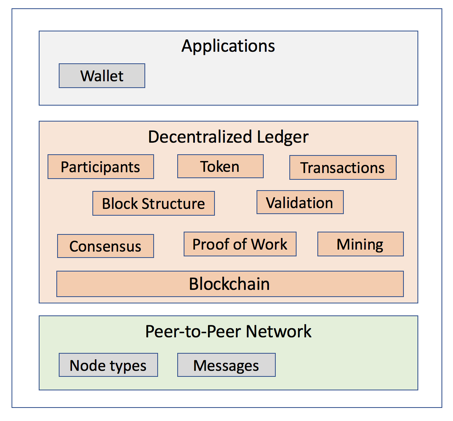
\includegraphics{figures/blockchain_architecture}
  \caption{Blockchain architectuur}
  \label{architecture:blockchain_architecture}
\end{wrapfigure}

Deze vraag heb ik opgesteld ter identificatie van de componenten die betrekking hebben tot de segmenten Distributed Network en Identity Management. Allereerst heb ik gezocht naar een bron waarin een compleet overzicht van de architectuur van een Blockchain implementatie getoond wordt. Via google kwam ik op fig. \ref{architecture:blockchain_architecture} waarin een duidelijk overzicht te zien is van de verschillende lagen in een Blockchain. Door het beschrijven van elke laag is er goede onderkenning opgebouwd voor Blockchains die gebruik maken van Proof of Work.

\subsection{Resultaat}

In de applicatie laag is de wallet te vinden die een gebruiker van de Blockchain doorgaans gebruikt om transacties te verrichten. De onderliggende functionaliteit van de wallet doet niets meer als het bijhouden van public- en private keys van de gebruiker waarop de nog niet uitgegeven tokens (cryptocurrency, contracten, diensten) geregistreerd staan.

De Decentralized Ledger is de kern van de technologie en zorgt ervoor dat de globale blockchain consistent en fraudebestending blijft. De fundamentele structuur achter de gehele technologie is de blockchain, waar transacties gegroepeerd worden in blokken en elk blok cryptografisch verbonden wordt met het vorige blok. Een transactie is een vorm van uitwisseling van tokens tussen deelnemers, ook wel nodes genoemd, van het systeem. Voordat transacties als valide worden beschouwd, ondergaan ze een validatie proces die uitgevoerd wordt door alle nodes in het systeem. Het proces van het groeperen van transacties in een blok dat toegevoegd wordt aan het einde van de blockchain wordt ook wel minen genoemd. Om er zeker van te zijn dat er overeenstemming is onder alle deelnemers over welke blockchain legitiem is, wordt er gebruik gemaakt van een Proof-of-Work algoritme tijdens het mining proces om te bepalen welke ketting de meeste inspanning vereist.

Het laatste component is het peer-to-peer netwerk, waarin verschillende node types gedefinieerd zijn. Zo heb je bijvoorbeeld de validatie node die transacties valideert en een mining node die het mining process uitvoert. Om de Decentralized Ledger bij te werken en te onderhouden communiceren de nodes met elkaar door middel van het versturen van berichten.

\subsection{Conclusie}

Het antwoord op de vraag ``\textbf{Uit welke componenten bestaan een Blockchain implementatie}'' is dan ook het volgende:

Een Blockchain bestaat uit meerdere lagen met daarin verschillende componenten. Zo heb je de applications laag waarin de wallet te vinden is die de public- en private key van de gebruiker beheerd. De laag Decentralized Ledger bevat de kern van de Blockchain technologie, waarin de componenten transacties, het consensus protocol, en de uiteindelijke Blockchain te vinden is. Als laatste is er de Peer-to-Peer Network laag, waarin de verschillende node types te vinden zijn. Ook is hier te vinden hoe berichten verstuurd worden naar ondelinge participanten van het netwerk.

Uit deze vraag heb ik een goed overzicht gekregen van wat de Blockchain technologie inhoudt. Ook geeft deze vraag inzicht in wat er te vinden is in het Distributed Network segment, oftewel de Peer-to-Peer Network laag.

